\documentclass[11pt,a4paper]{article}
\usepackage[utf8]{inputenc}
\usepackage[left=2cm,text={18cm,24cm},top=2cm]{geometry}
\usepackage[czech]{babel}
\usepackage[IL2]{fontenc}
\usepackage{verbatim}
\usepackage{xcolor}
\usepackage{graphicx}



\begin{document}
\fontfamily{phv}\selectfont
\huge \textbf{\color{violet}Příloha: Výstupní zpráva}

\bigskip

\large \textbf{Jméno: Dmitrii Ivanushkin}

\large \textbf{Login: xivanu00}

\bigskip

\Large \textbf{\color{violet}Architektura navrženého obvodu (na úrovni RTL)}

\bigskip

\large \textbf{\color{violet}Schéma obvodu}

\bigskip

\begin{figure}[h]
    \centering
    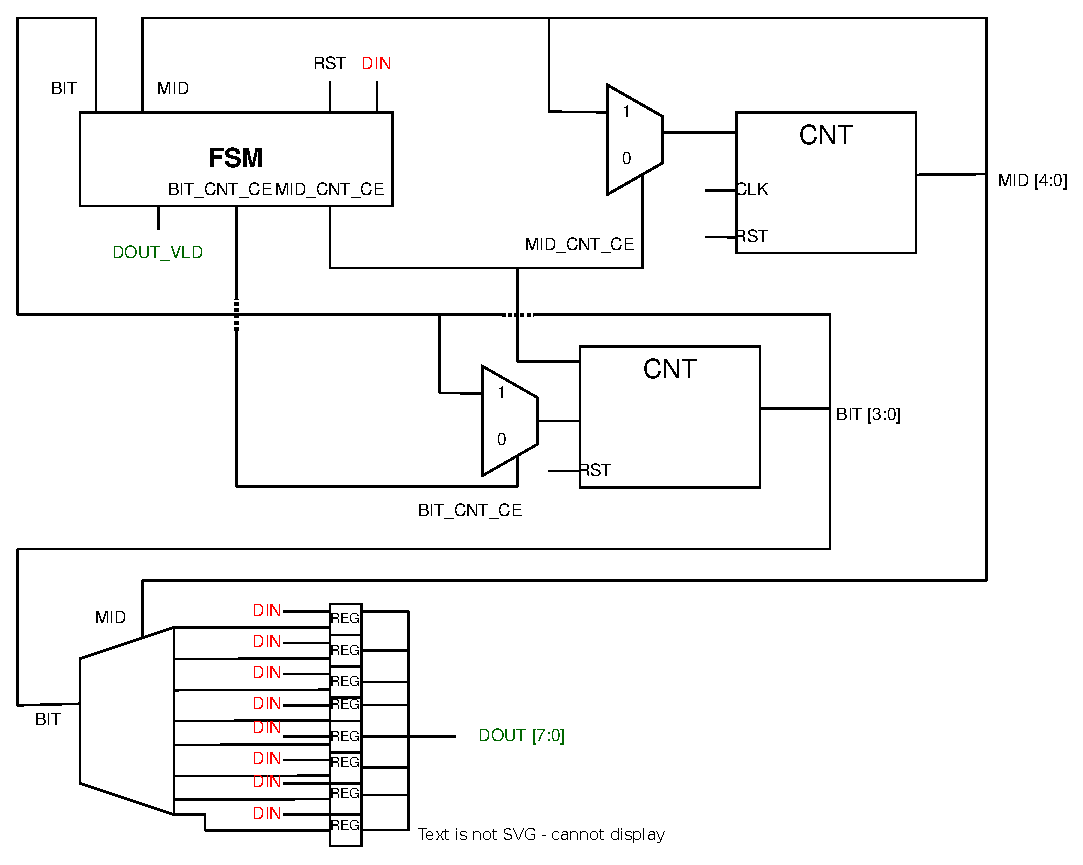
\includegraphics[scale=1]{pic1.eps}
\end{figure}

\newpage
\Large \textbf{\color{violet}Návrh automatu (Finite State Machine)}

\bigskip

\large \textbf{\color{violet}Schéma automatu}

\bigskip
Legenda:
\begin{itemize}
\setlength\itemsep{-1mm}
    \item[--] \quad Stavy automatu: \textsc{init, start, read, end}
    \item[--] \quad Vstupní signály: \textsc{D: DIN, M: MID, B: BIT}
    \item[--] \quad Mealyho výstupy: \textsc{MID\_CNT\_CE, BIT\_CNT\_CE, DOUT\_VLD}
\end{itemize}

\bigskip

\begin{figure}[h]
    \centering
    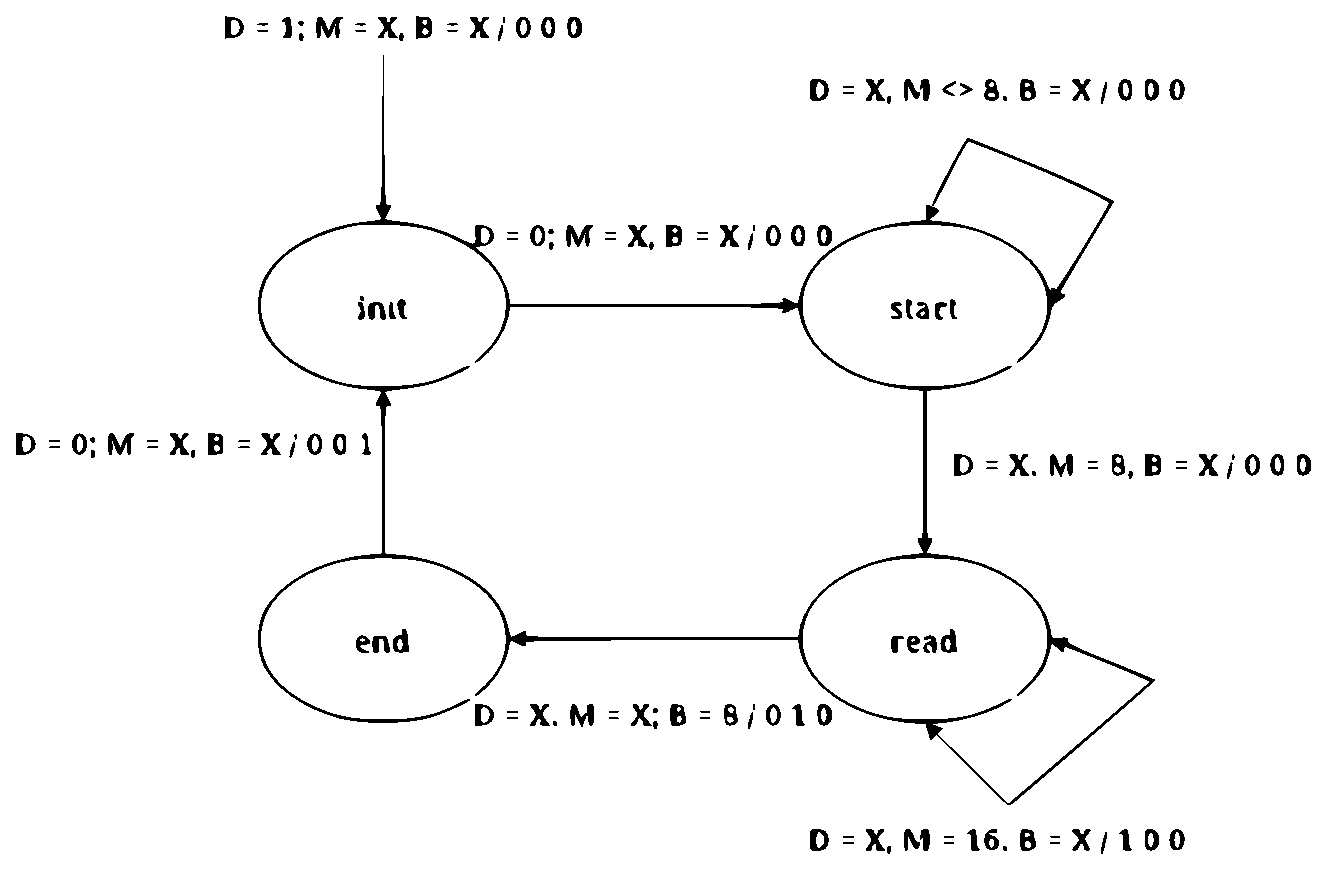
\includegraphics[scale=0.75]{pic2.eps}
\end{figure}

\Large \textbf{\color{violet}}

\bigskip

\large \textbf{\color{violet}Popis funkce}

\bigskip

FSM začíná svůj cyklus když má na vstupu DIN. Poté FSM počká na MID, který po 8 hodinovému cyklu pošle přejde do stavu read, a tam program bude čekat až MID se bude rovnat 16 (můžeme číst data, takže východ je MID\_CNT\_CE) a přejdeme do stavu end s výstupem BIT\_CNT\_CE (máme nějaký bit). Ve stavu end pošleme na východ DOUT\_VLD a skončíme program (přejdeme do init až ynovu dostaneme DIN)

\end{document}
